\documentclass{article}
\usepackage{geometry}
\usepackage{flafter}
\geometry{letterpaper, portrait, margin=1in}

\usepackage{hyperref}
\hypersetup{
    colorlinks=true,
    linkcolor=black,
    filecolor=magenta,
    urlcolor=blue,
}
\usepackage{listings}
\lstdefinestyle{bashstyle}{
  language=bash,
  basicstyle=\ttfamily,
  keywordstyle=\color{blue},
  commentstyle=\color{green},
  numberstyle=\tiny\color{gray},
  numbers=left,
  breaklines=true
}

\usepackage{tikz} % Import the tikz package
\usetikzlibrary{automata} % Import library for drawing automata
\usetikzlibrary{positioning} % ...positioning nodes
\usetikzlibrary{arrows} % ...customizing arrows
\tikzset{node distance=2.5cm, % Minimum distance between two nodes. Change if necessary.
every state/.style={ % Sets the properties for each state
semithick,
fill=gray!10},
initial text={}, % No label on start arrow
double distance=2pt, % Adjust appearance of accept states
every edge/.style={ % Sets the properties for each transition
draw,
->,>=stealth', % Makes edges directed with bold arrowheads
auto,
semithick}}
\let\epsilon\varepsilon

\usepackage{graphicx}
\graphicspath{ {images/} }

\usepackage{tcolorbox}
\usepackage{textcomp}
\usepackage{gensymb}
\usepackage{indentfirst}

\newcommand{\ans}{$\rule{1.5cm}{0.15mm}$}

\title{RoboJackets Firmware Training Week 2 Lab Guide}
\author{Andrew Rocco, Andrew Roach}
\date{\today\\v1.1}

\begin{document}
\maketitle{}
\setcounter{tocdepth}{2}
\tableofcontents
\pagebreak

%Everything below is for you to edit. Code above sets up the general formatting for the document

\section{Background}
    \subsection{Topics}
        The important topics being discussed this week in lab include state machines, interrupts, and more complex C++.
    \subsection{Premise}
        The lab premise is to make a state machine that implements a simple counter. At the start of the program, the counter should start at 0 and should be able to count up to 5 and back down to 0. This state machine will change states based on the 2 button inputs and will display state using the 5 controllable LEDs. One button input will be able to increment and the other decrement.
    \subsection{Interrupt Service Routines}
        Interrupt Service Routines (ISR) are functions that are called when interrupts are activated. These are usually short functions that should be used to update variables in global scope. Remember that interrupts are when your microcontroller gets a signal that makes it stop whats its doing, run the ISR, and then return to the code it was running. Interrupt-based programming is very common for microcontrollers and robots and is usually more efficient that other methods.
        
    \subsection{Simulation}
        If you are using a simulation instead of the hardware, do not worry.  The steps are exactly the same.  Go to the TinkerCad link and you will see the circuit that is a subset of the the hardware. The Arduino you see will be what you use, with the LEDs and buttons replicated as they would be on the actual board. 
        
        \begin{figure}[ht]
            \centering
            \includegraphics[width = 0.7\textwidth]{images/TinkerCadWires.png}
            \caption{The circuit window of TinkerCAD for this project}
        \end{figure}
        
        \begin{figure}[ht]
            \centering
            \includegraphics[width = 0.7\textwidth]{images/TinkerCadCode.png}
            \caption{The area which you can use to select your target and compile}
        \end{figure}
    
    \subsection{Firmware Training Board}
    If you are using the hardware, there are a few steps to complete to ensure that you can program the Arduino Nano on the circuit board. You may need to download the CH340 driver for your operating system which can be found \href{https://learn.sparkfun.com/tutorials/how-to-install-ch340-drivers/all}{here}. If you completed this in Week 1 there is no need to do this again. Remember in Tools$>$Board Type, ensure that you have set the board to Arduino Nano. Also make sure that you have selected the correct COM port in Tools$>$Port. For these Arduino Nanos you also need to select Tools$>$Processor$>$ATmega328P (Old Bootloader). 
    
        

\section{Materials}
\begin{itemize}
	\item If running Simulation: \href{https://www.autodesk.com/education/edu-software/overview}{AutoDesk Education Account} and \href{https://www.tinkercad.com/things/8J1RA4SvqOM}{TinkerCAD}
	\item If running on Firmware Training Board: \href{https://github.com/RoboJackets/firmware-training/blob/master/code/Week2/Week_2_Template/Week_2_Template.ino}{Firmware Training Board Template Code} and \href{https://www.arduino.cc/en/software}{Arduino IDE}
\end{itemize}

\section{Objectives}
    \subsection{Task 1 - Create State Machine}
        \begin{enumerate}
            \item Plan and draw out the full state machine.
            \begin{itemize}
                \item Make sure you have all the states and transitions marked. 
                \item As a programming convention, we will number our states from 0 upwards, which you will find more useful in the next step.
                \item Don't forget that no LEDs can be on for our counter.
                \item A refresher on state machines and a template to get started can be found in Section \ref{statemachine}.
            \end{itemize}
            \item Write code to display state in \texttt{loop}.
            \begin{itemize}
                \item You will need to go through every LED to set it state, so use a \texttt{for} loop and the \texttt{pinArray} array.
                \item Make sure to use the fact your states are starting counting at 0, which is similar to arrays. 
                \item You will need to use your state variable to know how to do the update.
            \end{itemize}
        \end{enumerate}
    \subsection{Task 2 - Create Interrupts}
        \begin{enumerate}
            \item Write an ISR for each button.
            \begin{itemize}
                \item SW1 is a button that when pressed sends a \texttt{HIGH} value to the Arduino, but is otherwise \texttt{LOW}. You should make sure this button should increase the number of LEDs turned on. 
                \item SW2 is a button that when pressed sends a \texttt{LOW} value to the Arduino, but is otherwise \texttt{HIGH}. This button should decrease the number of LEDs turned on.
            \end{itemize}
            \item Write code in \texttt{setup} for the buttons and interrupts.
            \begin{itemize}
                \item You will also need to setup the buttons as normal digital inputs first. 
                \item Make sure to understand how each button has a different type of change, which will affect how the interrupt triggers.
                \item A refresher on setting up interrupts can be found in Section \ref{attachinterrupt}.
            \end{itemize}
        \end{enumerate}
        

\section{Relevant Information}
    \subsection{State Machines} \label{statemachine}
        State machines are tools to organize the behavior of code, based around a number of "states" or points the code can be at. We specifically are looking at state machines that have output behavior depend only on current state, meaning the number of behaviors equals the number of states. The state machine inputs are used to trigger transitions to different states, and there no transitions to an impossible state. A graphical representation is often used with bubbles representing states and labelled arrows representing transitions. In addition, a state-transition table can be used to show what state a finite-state machine will move to based on the input and current state. Templates for both the table and graphical representation are given with the first two transitions filled out.
        
        \begin{center}
            \begin{tabular}{|c|c|c|c|}
                \hline
                Current State & Input & Next State & LED Output \\
                \hline
                State 0 & SW2 = 0 & State 0 & 0 \\ 
                State 0 & SW1 = 1 & State 1 & 1 \\
                \hline
                State 1 & SW2 = 0 &  &  \\
                State 1 & SW1 = 1 &  &  \\
                \hline
                State 2 & SW2 = 0 &  &  \\
                State 2 & SW1 = 1 &  &  \\
                \hline
                State 3 & SW2 = 0 &  &  \\
                State 3 & SW1 = 1 &  &  \\
                \hline
                State 4 & SW2 = 0 &  &  \\
                State 4 & SW1 = 1 &  &  \\
                \hline
                State 5 & SW2 = 0 &  &  \\
                State 5 & SW1 = 1 &  &  \\
                \hline
            \end{tabular}
        \end{center}
        
        \begin{center}
            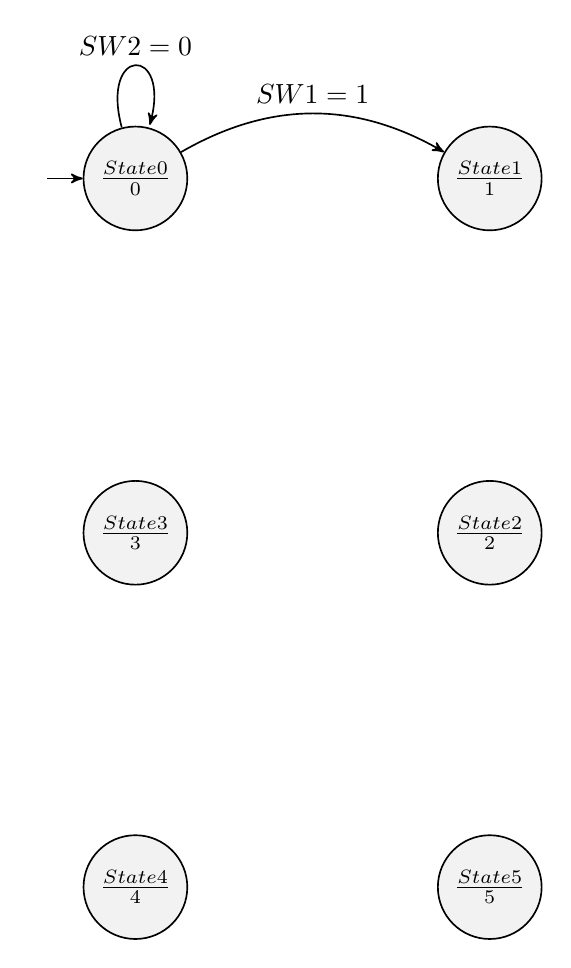
\begin{tikzpicture}
                \node[state, initial] (0) {$\frac{State 0}{0}$};
                \node[state, right of = 0, xshift=2cm] (1) {$\frac{State 1}{1}$};
                \node[state, below of = 0, yshift=-2cm] (3) {$\frac{State 3}{3}$};
                \node[state, right of = 3, xshift=2cm] (2) {$\frac{State 2}{2}$};
                \node[state, below of = 3, yshift=-2cm] (4) {$\frac{State 4}{4}$};
                \node[state, right of = 4, xshift=2cm] (5) {$\frac{State 5}{5}$};
                
                \draw (0) edge[loop above] node{$SW2 = 0$} (0)
                (0) edge[bend left, above] node{$SW1 = 1$} (1);
            \end{tikzpicture}
        \end{center}
        
        
        \begin{figure}[ht]
            \centering
            \includegraphics[width = 0.5\textwidth]{images/StateMachine.png}
            \caption{Example State Machine}
        \end{figure}
        
    \subsection{\texttt{attachInterrupt} Function} \label{attachinterrupt}
        The function we will be using for setting up interrupts is the \texttt{attachInterrupt} Function. You can refer to the reference page \href{https://www.arduino.cc/reference/en/language/functions/external-interrupts/attachinterrupt}{here} for understanding it along with examples. Specifically, you need to look into how to convert a pin to a interrupt number and to set the mode that triggers the interrupts. Note that you should use the recommended syntax using the \texttt{digitalPinToInterrupt} function.
        
        \begin{figure}[ht]
            \centering
            \includegraphics[width = 0.75\textwidth]{images/AttachInterrupt.png}
            \caption{\texttt{attachInterrupt} Function on the Arduino Website}
        \end{figure}
        

\section{Troubleshooting}
    \subsection{Solutions}
    We have included the solutions below if you do not complete the lab during the session or if you want to verify your answer. If you need help during the lab ask an instructor!
\begin{itemize}
    \item \href{https://www.tinkercad.com/things/cGKh5f8nkDv}{TinkerCAD Solution}
    \item \href{https://github.com/RoboJackets/firmware-training/blob/master/code/Week2/Week_2_Solution/Week_2_Solution.ino}{Firmware Training Board Template Solution}
    \item State Machine Solution
    \begin{center}
            \begin{tabular}{|c|c|c|c|}
                \hline
                Current State & Input & Next State & LED Output \\
                \hline
                State 0 & SW2 = 0 & State 0 & 0 \\ 
                State 0 & SW1 = 1 & State 1 & 1 \\
                \hline
                State 1 & SW2 = 0 & State 0 & 0 \\
                State 1 & SW1 = 1 & State 2 & 2 \\
                \hline
                State 2 & SW2 = 0 & State 1 & 1 \\
                State 2 & SW1 = 1 & State 3 & 3 \\
                \hline
                State 3 & SW2 = 0 & State 2 & 2 \\
                State 3 & SW1 = 1 & State 4 & 4 \\
                \hline
                State 4 & SW2 = 0 & State 3 & 3 \\
                State 4 & SW1 = 1 & State 5 & 5 \\
                \hline
                State 5 & SW2 = 0 & State 4 & 4 \\
                State 5 & SW1 = 1 & State 5 & 5 \\
                \hline
            \end{tabular}
        \end{center}
        
        \begin{center}
            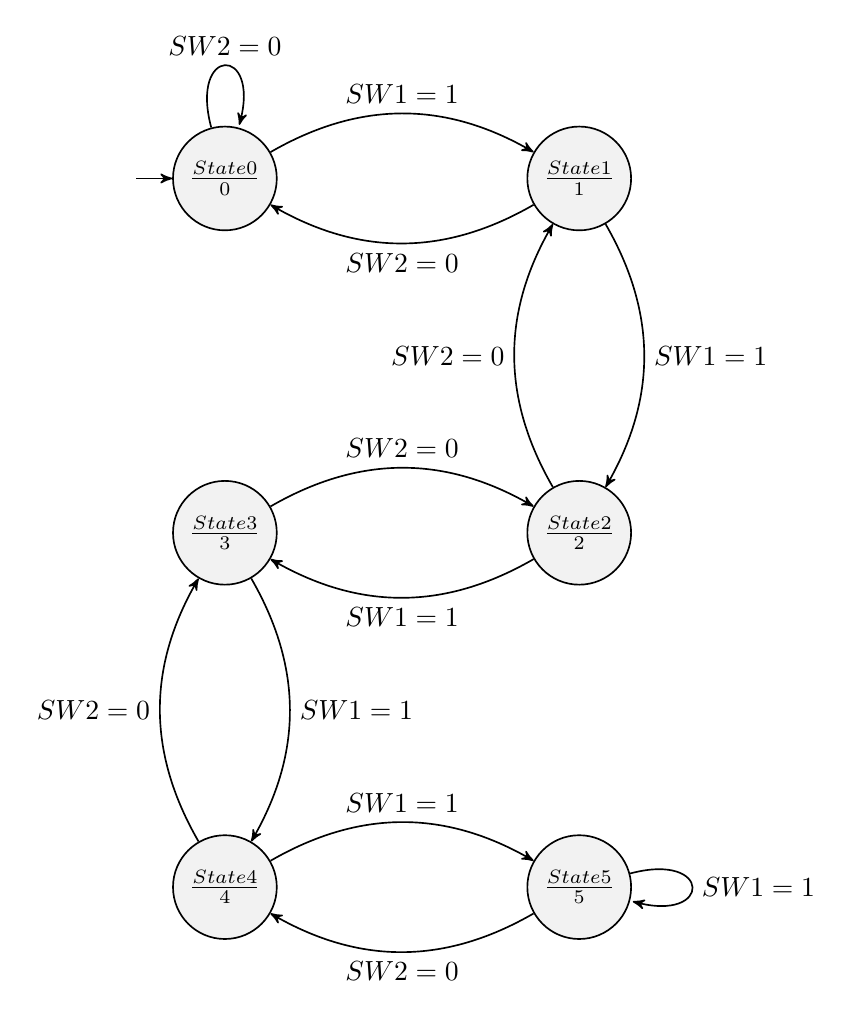
\begin{tikzpicture}
                \node[state, initial] (0) {$\frac{State 0}{0}$};
                \node[state, right of = 0, xshift=2cm] (1) {$\frac{State 1}{1}$};
                \node[state, below of = 0, yshift=-2cm] (3) {$\frac{State 3}{3}$};
                \node[state, right of = 3, xshift=2cm] (2) {$\frac{State 2}{2}$};
                \node[state, below of = 3, yshift=-2cm] (4) {$\frac{State 4}{4}$};
                \node[state, right of = 4, xshift=2cm] (5) {$\frac{State 5}{5}$};
                
                \draw (0) edge[loop above] node{$SW2 = 0$} (0)
                (0) edge[bend left, above] node{$SW1 = 1$} (1)
                (1) edge[bend left, below] node{$SW2 = 0$} (0)
                (1) edge[bend left, right] node{$SW1 = 1$} (2)
                (2) edge[bend left, left] node{$SW2 = 0$} (1)
                (2) edge[bend left, below] node{$SW1 = 1$} (3)
                (3) edge[bend left, above] node{$SW2 = 0$} (2)
                (3) edge[bend left, right] node{$SW1 = 1$} (4)
                (4) edge[bend left, left] node{$SW2 = 0$} (3)
                (4) edge[bend left, above] node{$SW1 = 1$} (5)
                (5) edge[bend left, below] node{$SW2 = 0$} (4)
                (5) edge[loop right] node{$SW1 = 1$} (5);


            \end{tikzpicture}
        \end{center}
        
        
    \end{itemize}

\newpage

\section{Appendix}

\subsection{Installing the Arduino IDE}

We will be using the legacy version of the Arduino IDE (version 1.8.19). Follow the installation instructions based on your platform.

\subsubsection{Windows and Mac}

\begin{enumerate}
    \item Go to the \href{https://www.tinkercad.com/things/cGKh5f8nkDv}{Arduino Software} page and scroll down to the ``Legacy IDE (1.8.X)''. Download the binary corresponding to your platform.
    \item Run the installer. Allow the installer to install everything, including drivers.
\end{enumerate}

\subsubsection{Linux}

\begin{enumerate}
    \item Go to the \href{https://www.tinkercad.com/things/cGKh5f8nkDv}{Arduino Software} page and scroll down to the ``Legacy IDE (1.8.X)''. The Linux Arduino IDE should download as a \verb|tar.xz| file.
    \item Run the following commands, replacing \verb|<arduino-ide>| with the name of the downloaded file.
    \begin{lstlisting}[style=bashstyle, label=lst:mybashcode]
    tar -xJvf <arduino-ide>.tar.xz -C /home/$(whoami)
    cd /home/$(whoami)/<arduino-ide>
    sudo ./install.sh
    \end{lstlisting}
\end{enumerate}

\subsection{Verify CH340 Drivers}

Our Arduino Nanos are kinda old, so they often don't work out of the box without installing the correct drivers first. Your operating system or the installation of the Arduino IDE might have installed the correct drivers, so it's a good idea to check if you have the driver before reinstalling them.

\subsubsection{Windows}

{\bf Checking if driver is present: } type \verb|driverquery| into the command prompt. You should see a driver called \verb|CH341SER|. 

\vspace{1em}

{\bf Checking if driver loads: } Plug the Arduino Nano into your computer. Go to \verb|Device Manager| and look under \verb|Ports|. You should see the Arduino Nano as \verb|USB-SERIAL CH340|, followed by the \verb|COM| port it's associated with.

\subsubsection{Linux}

{\bf Checking if module is present: } type \verb|modinfo ch341| into your shell. The command should return a bunch of information about the \verb|ch341| kernel module.

\vspace{1em}

{\bf Checking if driver is present: } Plug the Arduino Nano into your computer. Enter the command \verb|sudo dmesg| into your shell.

\begin{itemize}
    \item If you see the following, you need to uninstall \verb|br1tty|. After uninstalling \verb|br1tty|, unplug and plug in the Arduino Nano and run \verb|sudo dmesg| again.
    \begin{itemize}
        \item Ubuntu: \verb|sudo apt remove br1tty|.
    \end{itemize}
    \item If you see the following, type \verb|ls /dev/tty*|. You should see the Arduino Nano show up as \verb|/dev/ttyUSB[0-9]| or \verb|/dev/ttyACM[0-9]|. This indicates that the kernel module has loaded successfully.

\end{itemize}


\newpage

\subsection{Install CH340 Drivers}

If you could not find the \verb|CH340| drivers, you may have to install them manually.

\subsubsection{Windows and Mac}

Follow the instructions 


\end{document}